\documentclass{article}

\usepackage{graphicx}
\usepackage{float}
\usepackage{caption}
\usepackage{subcaption}

\usepackage{array}
\newcolumntype{L}[1]{>{\raggedright\let\newline\\\arraybackslash\hspace{0pt}}m{#1}}
\newcolumntype{C}[1]{>{\centering\let\newline\\\arraybackslash\hspace{0pt}}m{#1}}
\newcolumntype{R}[1]{>{\raggedleft\let\newline\\\arraybackslash\hspace{0pt}}m{#1}}

\begin{document}

\begin{figure}[H]
    \centering
    \captionsetup{justification=centering, size=scriptsize}
    \begin{subfigure}{0.45\textwidth}
      \includegraphics[width=1\textwidth]{pictures/ small_cycle_with_agents.png}
      \caption{Small cycle}
      \scriptsize
      \begin{tabular}{ | L{2 cm} | L{0.5 cm} | }
      \hline
      Agents & 3  \\ \hline
      Works & 3  \\ \hline
      Items & 6  \\ \hline
      \end{tabular}
      \label{fig:cycle-small-with-agents}
    \end{subfigure}
    \quad
    \begin{subfigure}{0.38\textwidth}
      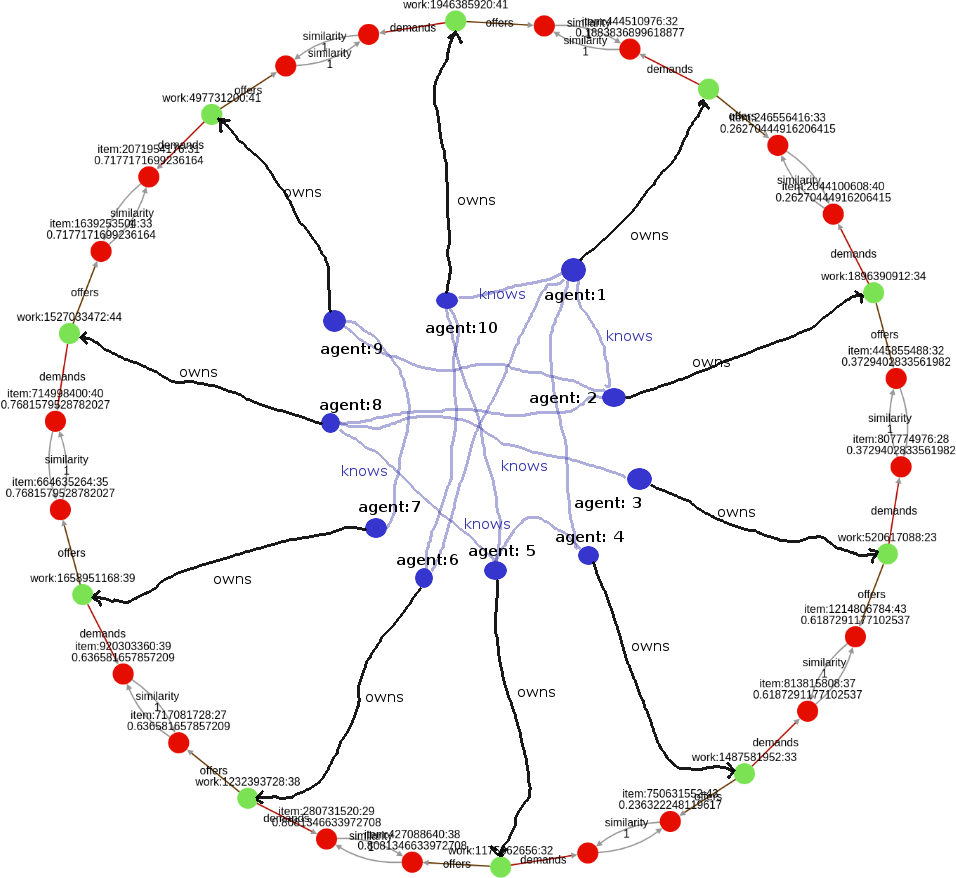
\includegraphics[width=1\textwidth]{pictures/larger_cycle_with_agents.png}
      \caption{Larger cycle}
      \scriptsize
      \begin{tabular}{ | L{2 cm} | L{0.5 cm} | }
      \hline
      Agents & 10  \\ \hline
      Works & 10  \\ \hline
      Items & 20  \\ \hline
      \end{tabular}
      \label{fig:cycle-larger-with-agents}
    \end{subfigure}
    \footnotesize
    \caption{Cycles discovered in the OfferNet(s) graph by cycle search processes.}
    \label{fig:cycle-search}
\end{figure}

\end{document}